Ud fra applikationsmodellens klasse diagram (Figur \ref{fig:CSS_hovedenhed_Class}) og en dybere analyse af funktionalitete er der udledt et statisk klassediagram, se figur \ref{fig:CSS_hovedenhed_Class_Static}. Dette baserer sig på analyse og praktisk implementering.

\begin{figure}[!htb] \centering
     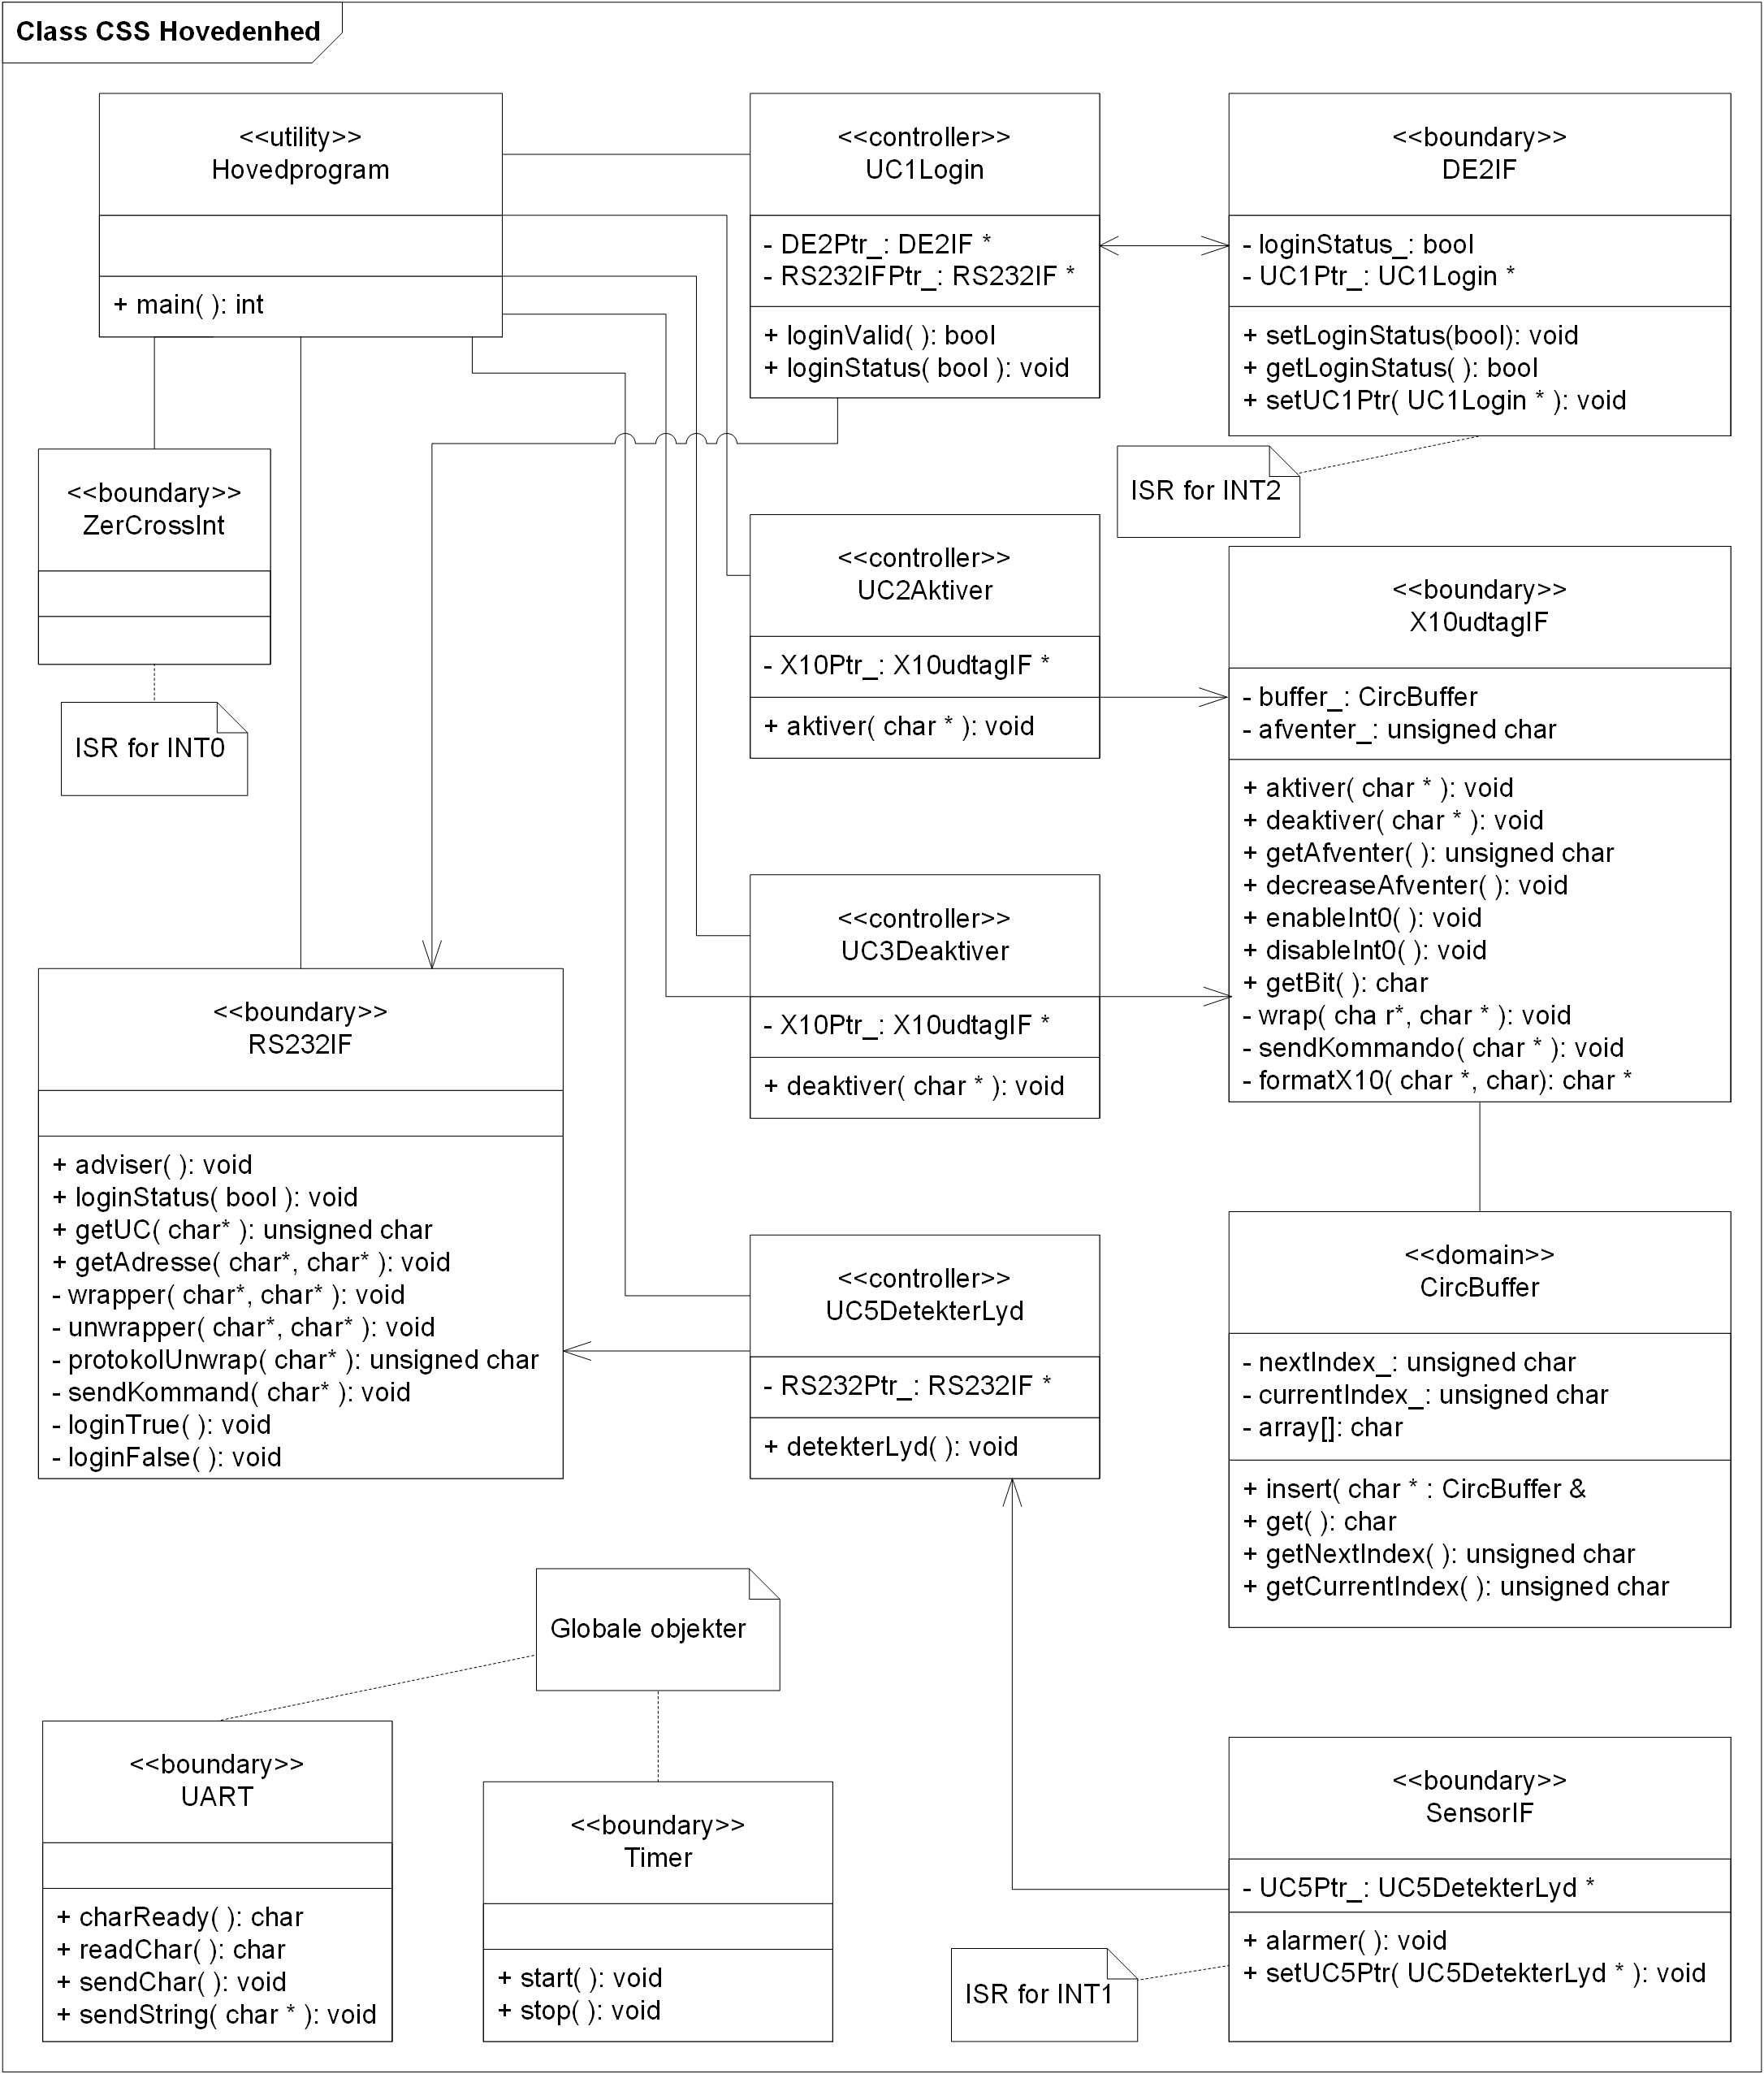
\includegraphics[width=\textwidth]{billeder/uml/CSS_hovedenhed_Class_Static}
     \caption{Statisk klassediagram for CSS hovedenhed}
     \label{fig:CSS_hovedenhed_Class_Static}
\end{figure}
	
Her følger klassebeskrivelser for alle klasser til CSS hovedenheden. \\

%
% RS232IF
%
{\centering
\textbf{RS232IF}\par
}
\textbf{Ansvar:} At varetage kommunikation mellem CSS hovedenhed og PC over RS232 protokollen. \\
\textbf{Attributer:} Ingen \\
\textbf{Metoder:} \\
void adviser(); \\
\textbf{Parametre:} Ingen \\
\textbf{Returværdi:} Ingen \\
\textbf{Beskrivelse:} Sender kommando "SB9999\textbackslash r" over RS232 forbindelsen \\

void loginStatus( bool status ); \\
\textbf{Parametre:} Status for login, true = logget ind, false = logget ud  \\
\textbf{Returværdi:} Ingen \\
\textbf{Beskrivelse:} Kalder hjælpemetoderne loginTrue() eller loginFalse() afhængig af status parameteren \\

unsigned char getUC( char * kommando ); \\
\textbf{Parametre:} Pointer med plads til den modtagende RS232 kommando \\
\textbf{Returværdi:} Nummer på UC som tal \\
\textbf{Beskrivelse:} Afventer en fuld data pakke på RS232 forbindelsen. Gemmer den ud fra pointeren. Dekoder kommandoen iht. RS232 protokollen og returnerer UC nummeret \\

void getAdresse( char * kommando, char * adresse); \\
\textbf{Parametre:} Pointer til den modtagede kommando. Pointer med plads til adressen. \\
\textbf{Returværdi:} Ingen \\
\textbf{Beskrivelse:} Hvis kommandoen er formateret med STX og ETX fjernes disse og adressen skrives over i adresse pointeren \\

void wrapper( const char * kommando, char * wrapped); \\
\textbf{Parametre:} Pointer til rå kommando data uden STX og ETX. Pointer med plads til den fulde kommando inkl. STX og ETX \\
\textbf{Returværdi:} Ingen \\
\textbf{Beskrivelse:} Indsætter STX og ETX karaktere iht. RS232 protokollen\\

void unWrapper( const char * wrapped, char * kommando); \\
\textbf{Parametre:} Pointer til rå kommando data inkl. STX og ETX. Pointer med plads til kommandoen uden STX og ETX \\
\textbf{Returværdi:} Ingen \\
\textbf{Beskrivelse:} Fjerner STX og ETX karaktere iht. RS232 protokollen\\

unsigned char protokolUnwrap( char * kommando); \\
\textbf{Parametre:} Pointer til rå kommando data uden STX og ETX \\
\textbf{Returværdi:} Ingen \\
\textbf{Beskrivelse:} Returnerer et tal svarende til UC nummeret ud fra RS232 protokollen \\

void sendKommando( char * wrapped ); \\
\textbf{Parametre:} Pointer til rå kommando data inkl. STX og ETX \\
\textbf{Returværdi:} Ingen \\
\textbf{Beskrivelse:} Sender hvert tegn i kommandoen, igennem det globale RS232UART objekt, ud på RS232 forbindelsen\\

void loginTrue(); \\
\textbf{Parametre:} Ingen \\
\textbf{Returværdi:} Ingen \\
\textbf{Beskrivelse:} Sender kommando ''ST9999\textbackslash r'' over RS232 forbindelsen\\

void loginFalse(); \\
\textbf{Parametre:} Ingen \\
\textbf{Returværdi:} Ingen \\
\textbf{Beskrivelse:} Sender kommando ''SF9999\textbackslash r'' over RS232 forbindelsen\\

%
% UC1Login
%
{\centering
\textbf{UC1Login}\par
}
\textbf{Ansvar:} At varetage UC1 Login forløbet. \\
\textbf{Attributer:}
\begin{itemize}
	\item \textbf{DE2IF * DE2Ptr\_} \\
	Pointer til associeret DE2IF objekt
	\item \textbf{RS232IF * RS232IFPtr\_} \\
	Pointer til associeret RS232IF objekt
\end{itemize}
\textbf{Metoder:} \\
bool loginValid(); \\
\textbf{Parametre:} Ingen \\
\textbf{Returværdi:} True = logget ind, False = logget ud \\
\textbf{Beskrivelse:} Kalder getLoginStatus() metoden i DE2IF objektet og returnerer værdien her fra \\

void loginStatus( bool status ); \\
\textbf{Parametre:} True = logget ind, False = logget ud \\
\textbf{Returværdi:} Ingen \\
\textbf{Beskrivelse:} Kalder loginStatus() metoden i RS232IF objektet \\

%
% UC2Aktiver
%
{\centering
\textbf{UC2Aktiver}\par
}
\textbf{Ansvar:} At varetage UC2 Aktiver forløbet. \\
\textbf{Attributer:}
\begin{itemize}
	\item \textbf{X10IF * X10IFPtr\_} \\
	Pointer til associeret X10IF objekt
\end{itemize}
\textbf{Metoder:} \\
void aktiver( char * adresse ); \\
\textbf{Parametre:} Pointer til adressen på enhed \\
\textbf{Returværdi:} Ingen \\
\textbf{Beskrivelse:} Kalder aktiver() metoden i X10IF objektet med den modtagede adresse \\

%
% UC3Deaktiver
%
{\centering
\textbf{UC3Deaktiver}\par
}
\textbf{Ansvar:} At varetage UC3 Deaktiver forløbet. \\
\textbf{Attributer:}
\begin{itemize}
	\item \textbf{X10IF * X10IFPtr\_} \\
	Pointer til associeret X10IF objekt
\end{itemize}
\textbf{Metoder:} \\
void deaktiver( char * adresse ); \\
\textbf{Parametre:} Pointer til adressen på enhed \\
\textbf{Returværdi:} Ingen \\
\textbf{Beskrivelse:} Kalder deaktiver() metoden i X10IF objektet med den modtagede adresse \\

%
% UC5DetekterLyd
%
{\centering
\textbf{UC5DetekterLyd}\par
}
\textbf{Ansvar:} At varetage UC5 Detekter Lyd. \\
\textbf{Attributer:}
\begin{itemize}
	\item \textbf{RS232IF * RS232Ptr\_} \\
	Pointer til associeret RS232IF objekt
\end{itemize}
\textbf{Metoder:} \\
void detekterLyd(); \\
\textbf{Parametre:} Ingen \\
\textbf{Returværdi:} Ingen \\
\textbf{Beskrivelse:} Kalder adviser() metoden i RS232IF objektet \\

%
% DE2IF
%
{\centering
\textbf{DE2IF}\par
}
\textbf{Ansvar:} At holde styr på aktuel loginstatus på DE2 boardet.

Dette er en global klasse da ISR for INT2 benet kalder setLoginStatus() metoden. Det globale objekt hedder DE2IFObj. \\
\textbf{Attributer:}
\begin{itemize}
	\item \textbf{bool loginStatus\_} \\
	True = Login bekræftet på DE2 board \\
	False = Login ikke bekræftet på DE2 board
	\item \textbf{UC1Login * UC1Ptr\_} \\
	Pointer til associeret UC1Login objekt
\end{itemize}

\textbf{Metoder:} \\
void setLoginStatus( bool status ); \\
\textbf{Parametre:} True hvis logget ind, False hvis logget ud \\
\textbf{Returværdi:} Ingen \\
\textbf{Beskrivelse:} Sætter attribut loginStatus\_ til aktuel status på DE2 board og kalder endten start()- eller stop()-metoden i det globale loginTimer objekt hvis status er hendholdsvis true eller false \\

bool getLoginStatus(); \\
\textbf{Parametre:} Ingen \\
\textbf{Returværdi:} True hvis logget ind, False hvis logget ud \\
\textbf{Beskrivelse:} Returnerer attribut loginStatus\_ \\

void setUC1Ptr( UC1Login * Ptr ); \\
\textbf{Parametre:} Pointer til associeret UC1Login objekt \\
\textbf{Returværdi:} Ingen \\
\textbf{Beskrivelse:} Sætter pointer attribut til Ptr \\

ISR( INT2\_vect ); \\
\textbf{Parametre:} Adresse til INT2 vectoren \\
\textbf{Returværdi:} Ingen \\
\textbf{Beskrivelse:} Kald setLoginStatus() metoden med parameter true \\


%
% X10IF
%
{\centering
\textbf{X10IF}\par
}
\textbf{Ansvar:} At varetage kommunikation mellem CSS hovedenhed og X10 modtager over X10 protokollen.

Dette er en global klasse da ISR for INT0 tilgår buffer\_ objektet. Det globale objekt hedder X10IFObj. \\
\textbf{Attributer:}
\begin{itemize}
	\item \textbf{CircBuffer buffer\_} \\
	CircBuffer obejkt til at holde kommandoer inden afsendelse
	\item \textbf{unsigned char afventer\_} \\
	Holder antallet af kommandoer der venter på at blive afsendt. Kun positive tal
\end{itemize}
\textbf{Metoder:} \\
void aktiver( char * adresse ); \\
\textbf{Parametre:} Pointer til adresse på enhed der skal aktiveres \\
\textbf{Returværdi:} Ingen \\
\textbf{Beskrivelse:} Afsend kommandoen ''SAXXXX\textbackslash r'', hvor XXXX er adressen på enheden der skal aktiveres, over X10 forbindelsen ved brug af sendKommando() metoden \\

void deaktiver( char * adresse ); \\
\textbf{Parametre:} Pointer til adresse på enhed der skal deaktiveres \\
\textbf{Returværdi:} Ingen \\
\textbf{Beskrivelse:} Afsend kommandoen ''SDXXXX\textbackslash r'', hvor XXXX er adressen på enheden der skal deaktiveres, over X10 forbindelsen ved brug af sendKommando() metoden \\

unsigned char getAfventer( ); \\
\textbf{Parametre:} Ingen \\
\textbf{Returværdi:} Ingen \\
\textbf{Beskrivelse:} Returner afventer\_ attributen \\

void decreaseAfventer( ); \\
\textbf{Parametre:} Ingen \\
\textbf{Returværdi:} Ingen \\
\textbf{Beskrivelse:} Hvis afventer\_ ikker er 0 trækkes 1 fra \\

void enableInt0( ); \\
\textbf{Parametre:} Ingen \\
\textbf{Returværdi:} Ingen \\
\textbf{Beskrivelse:} Aktiver interrupts for INT0 benet ved toggles og aktiver global interrupt flag \\

void disableInt0( ); \\
\textbf{Parametre:} Ingen \\
\textbf{Returværdi:} Ingen \\
\textbf{Beskrivelse:} Deaktiver interrupts for INT0 benet \\

char getBit( ); \\
\textbf{Parametre:} Ingen \\
\textbf{Returværdi:} Ingen \\
\textbf{Beskrivelse:} Hent næste karakter i buffer\_ objektet med metogen get() \\

void wrap( char * unwrapped, char * wrapped ); \\
\textbf{Parametre:} Pointer til rå kommando uden STX og ETX. Pointer med plads til X10 formateret kommando \\
\textbf{Returværdi:} Ingen \\
\textbf{Beskrivelse:} Omskriv kommando fra RS232 format (''SAXXXX\textbackslash r'') til X10 format inkl. STX og ETX iht. X10 protokollen \\

void sendKommando( char * unwrapped ); \\
\textbf{Parametre:} Pointer til kommando i RS232 format (''SAXXXX\textbackslash r'') uden STX og ETX \\
\textbf{Returværdi:} Ingen \\
\textbf{Beskrivelse:} Omformater kommando til X10 format og indsæt i buffer\_ objektet. Terminer bufferen med '\textbackslash n'. Forøg afventer\_ attributen og aktiver interrupts på INT0 \\

char * formatX10( char * plads, char bit ); \\
\textbf{Parametre:} Pointer med plads til X10 formateret bit (2 char plader). Char som skal formateres fra. Kun '0' og '1' gyldige. \\
\textbf{Returværdi:} Pointer til næste plads i X10 kommando \\
\textbf{Beskrivelse:} Formaterer bit om til X10 formaterede bits iht. X10 protokollen og returnerer *plads + 2 \\

%
% CircBuffer
%
{\centering
\textbf{CircBuffer}\par
}
\textbf{Ansvar:} At holde kommandoer som ligger i kø til afsendelse. \\
\textbf{Attributer:}
\begin{itemize}
	\item \textbf{unsigned char nextIndex\_} \\
	Index til næste plads til skrivning
	\item \textbf{unsigned char currentIndex\_} \\
	Index til næste plads til læsning
	\item \textbf{char array[]} \\
	Array til at holde bit karakterende
\end{itemize}

\textbf{Metoder:} \\
CircBuffer( ); (Constructor)\\
\textbf{Parametre:} Ingen \\
\textbf{Returværdi:} Ingen \\
\textbf{Beskrivelse:} Initialiser attributter til 0. Fyld array med '\textbackslash 0' \\

CircBuffer \& insert( char * bit ); \\
\textbf{Parametre:} Pointer til bit der skal indsættes i bufferen \\
\textbf{Returværdi:} Reference til objektet (this) \\
\textbf{Beskrivelse:} Indsætter værdi i bufferen og ligger en til nextIndex\_ atributten. Hvis denne er større end arrayets størrelse startes fra 0\\

char get( ); \\
\textbf{Parametre:} Ingen \\
\textbf{Returværdi:} Udlæst bit fra arrayet \\
\textbf{Beskrivelse:} Udlæser bit fra arrayet. Ligger en til currentIndex\_ atributten. Hvis denne er større end arrayets størrelse startes fra 0\\

unsigned char getNextIndex( ); \\
\textbf{Parametre:} Ingen \\
\textbf{Returværdi:} Attributten nextIndex\_ \\
\textbf{Beskrivelse:} Returnerer attributten nextIndex\_ \\

unsigned char getCurrentIndex( ); \\
\textbf{Parametre:} Ingen \\
\textbf{Returværdi:} Attributten currentIndex\_ \\
\textbf{Beskrivelse:} Returnerer attributten currentIndex\_ \\

%
% SensorIF
%
{\centering
\textbf{SensorIF}\par
}
\textbf{Ansvar:} At holde styr på aktuel lyd detektering og give besked over RS232 forbindelsen hvis lyd registreres.

Dette er en global klasse da ISR for INT1 tilgår alarmer() metoden. Det globale objekt hedder SensorIFObj. \\
\textbf{Attributer:}
\begin{itemize}
	\item \textbf{UC5DetekterLyd * UC5Ptr\_} \\
	Pointer til associeret UC5 objekt
\end{itemize}

\textbf{Metoder:} \\
void alarmer( ); \\
\textbf{Parametre:} Ingen \\
\textbf{Returværdi:} Ingen \\
\textbf{Beskrivelse:} Kalder detekterLyd() metoden i UC5DetekterLyd objektet. \\

void setUC5Ptr( UC5DetekterLyd * Ptr ); \\
\textbf{Parametre:} Pointer til associeret UC5DetekterLyd objekt \\
\textbf{Returværdi:} Ingen \\
\textbf{Beskrivelse:} Initialiser UC5Ptr\_ til Ptr \\

ISR( INT1\_vect ); \\
\textbf{Parametre:} Adresse til INT1 vector \\
\textbf{Returværdi:} Ingen \\
\textbf{Beskrivelse:} Kald alarmer() metoden i det globale SensorIFObj objekt \\

%
% ZeroCrossInt
%
{\centering
\textbf{ZeroCrossInt}\par
}
\textbf{Ansvar:} At detekterer ZeroCross signalet og afsende X10 kommandoer ud fra dette.\\
\textbf{Attributer:} Ingen
\textbf{Metoder:} \\
ZeroCrossInt( ); (Constructor) \\
\textbf{Parametre:} Ingen \\
\textbf{Returværdi:} Ingen \\
\textbf{Beskrivelse:} Aktiver interrupts for INT0 og aktiver det globale interrupt flag \\

\~ZeroCrossInt( ); (Destructor) \\
\textbf{Parametre:} Ingen \\
\textbf{Returværdi:} Ingen \\
\textbf{Beskrivelse:} Deaktiver interrupts for INT0 \\

ISR( INT0\_vect ); \\
\textbf{Parametre:} Adresse til INT0 vector \\
\textbf{Returværdi:} Ingen \\
\textbf{Beskrivelse:} Hvis der er data i køen på X10IFObj objektet udhentes et bit fra den. Bittet afsendes ved at tænde for det globale Timer objekt iht. X10 protokollen. Hvis kommando termineringen udtages fra bufferen tælles køen ned. Hvis køen er tom deaktiveres interruptet ved at kalde disbaleInt0() metoden i X10IFObj objektet. \\

%
% UART
%
{\centering
\textbf{UART}\par
}
\textbf{Ansvar:} At interface med USART hardwaren på atMega32 processoren på STK500 kittet.

Dette er en global klasse og det globale objekt hedder RS232UART \\
\textbf{Attributer:}
\begin{itemize}
	\item \textbf{char dataIn[]} \\
	Global: Array til at holde modtagede karakterer
	\item \textbf{unsigned char volatile dataCount} \\
	Global: Tæller til at registrer mængden af modtagende karakterer
	\item \textbf{unsigned char volatile commandReady} \\
	Global: Flag til registrering af fuldt modtaget kommando
\end{itemize}
\textbf{Metoder:} \\
UART( unsigned long BaudRate, unsigned char databit ); (Constructor) \\
\textbf{Parametre:} Buadrate. Mellem 110 og 115200. Antallet af databits. Mellem 5 og 9. \\
\textbf{Returværdi:} Ingen \\
\textbf{Beskrivelse:} Sæt de hardwarenære registre til kommunikation med USART delen af atMega32 processoren samt modtage interrupts \\

\~UART( ); (Destructor) \\
\textbf{Parametre:} Ingen \\
\textbf{Returværdi:} Ingen \\
\textbf{Beskrivelse:} Deaktiver USART afsendelse og modtagelse samt modtage interrupt \\

char charReady( ); \\
\textbf{Parametre:} Ingen \\
\textbf{Returværdi:} >0 hvis data modtaget \\
\textbf{Beskrivelse:} Returner > 0 hvis der er modtaget data, ellers 0 \\

char readChar( ); \\
\textbf{Parametre:} Ingen \\
\textbf{Returværdi:} Modtaget karakter \\
\textbf{Beskrivelse:} Afvent data modtagning og returner modtaget char \\

void sendChar( char tegn ); \\
\textbf{Parametre:} Karakter til afsendelse \\
\textbf{Returværdi:} Ingen \\
\textbf{Beskrivelse:} Afvent afsendelsesbuffer klar og send karakter \\

void sendString( char * streng ); \\
\textbf{Parametre:} Pointer til nul-termineret karakter streng \\
\textbf{Returværdi:} Ingen \\
\textbf{Beskrivelse:} Kald sendChar() metoden for hver karakter indtil nul-terminering \\

ISR( USART\_RXC\_vect ); \\
\textbf{Parametre:} Adresse til USART modtagnings vector \\
\textbf{Returværdi:} Ingen \\
\textbf{Beskrivelse:} Læs modtaget data ind i dataIn[] arrayet. Registrer om en fuldt modtaget og termineret kommando er modtaget. Hvis det er tilfældet nulstilles dataCount og commandReady flaget sættes. Hvis der er modtaget flerer karakterer end kommandolængeden og de ikke har rigtige STX og ETX nulstilles bufferen. Hvis intet af ovenstående udføres, øges dataCount med 1\\

%
% Timer
%
{\centering
\textbf{Timer}\par
}
\textbf{Ansvar:} At genererer 120 kHz firkant signal med intern hardware timer.

Dette er en global klasse da ISR for INT0 kan tilgå start() og stop() metoderne. Det globale objekt hedder timer. \\
\textbf{Attributer:} Ingen
\textbf{Metoder:} \\
Timer( ); (Constructor) \\
\textbf{Parametre:} Ingen \\
\textbf{Returværdi:} Ingen \\
\textbf{Beskrivelse:} Sæt output port og indstil hardware registrer til timer1 på atMega32 processoren til at genererer 120 kHz firkant signal \\

\~ZeroCrossInt( ); (Destructor) \\
\textbf{Parametre:} Ingen \\
\textbf{Returværdi:} Ingen \\
\textbf{Beskrivelse:} Afbryd hardware forbindelse til timeren og stop den. Sæt ouput ben lavt \\

void start( ); \\
\textbf{Parametre:} Ingen \\
\textbf{Returværdi:} Ingen \\
\textbf{Beskrivelse:} Sæt hardware forbindelse til output ben og start timer1 \\

void stop( ); \\
\textbf{Parametre:} Ingen \\
\textbf{Returværdi:} Ingen \\
\textbf{Beskrivelse:} Afbryd hardware forbindelse til timeren og stop den. Sæt ouput ben lavt \\

%
% LoginTimer
%
{\centering
\textbf{LoginTimer}\par
}
\textbf{Ansvar:} At holde styr på tiden siden sidste validerede login med den interne timer0 i atMega32 processoren.

Dette er en global klasse da ISR for timer0 overflows tilgår objektet. Det globale objekt hedder loginTimer. \\
\textbf{Attributer:}
\begin{itemize}
	\item \textbf{unsigned int ovfCount\_} \\
	Tæller til at holde antallet af overflows
\end{itemize}
\textbf{Metoder:} \\
Timer( ); (Constructor) \\
\textbf{Parametre:} Ingen \\
\textbf{Returværdi:} Ingen \\
\textbf{Beskrivelse:} Initialiser ovfCount\_ atributten til 0 og kald stop() metoden \\

\~ZeroCrossInt( ); (Destructor) \\
\textbf{Parametre:} Ingen \\
\textbf{Returværdi:} Ingen \\
\textbf{Beskrivelse:} Kald stop() metoden \\

void start( ); \\
\textbf{Parametre:} Ingen \\
\textbf{Returværdi:} Ingen \\
\textbf{Beskrivelse:} Start timer0 til længst mulige tidstagning og aktiver overflow interrupts samt det globale interrupt flag \\

void stop( ); \\
\textbf{Parametre:} Ingen \\
\textbf{Returværdi:} Ingen \\
\textbf{Beskrivelse:} Stop timer0 og deaktiver overflow interrupts \\

void inc( ); \\
\textbf{Parametre:} Ingen \\
\textbf{Returværdi:} Ingen \\
\textbf{Beskrivelse:} Tæl ovfCount\_ 1 op. Hvis den rammer overflow grænsen, som afgør tiden man er logget ind kaldes setLoginStatus() metoden i det globaleDE2IFObj objekt og ovfCount\_ nulstilles  \\

ISR( TIMER0\_OVF\_vect ); \\
\textbf{Parametre:} Adresse til timer0 overflow vectoren \\
\textbf{Returværdi:} Ingen \\
\textbf{Beskrivelse:} Kald inc() metoden i loginTimer objektet \\




